\documentclass[11pt,a4paper]{article}

\usepackage[margin=2.4cm]{geometry}
\usepackage[T1]{fontenc}
\usepackage{lmodern}
\usepackage{microtype}
\usepackage{amsmath,amssymb}
\usepackage{graphicx}
\usepackage{booktabs}
\usepackage{array}
\usepackage{xcolor}
\usepackage{enumitem}
\usepackage[font=small,labelfont=bf]{caption}
\usepackage{listings}
\usepackage[colorlinks=true,linkcolor=blue!60!black,citecolor=blue!60!black,urlcolor=blue!60!black]{hyperref}

\setlist{itemsep=2pt,topsep=4pt}
\setlength{\parskip}{4pt}
\setlength{\parindent}{0pt}

\definecolor{codebg}{RGB}{246,246,246}
\lstset{
  basicstyle=\ttfamily\footnotesize,
  backgroundcolor=\color{codebg},
  frame=single, rulecolor=\color{black!20},
  breaklines=true, breakatwhitespace=false,
  columns=fullflexible, keepspaces=true,
  showstringspaces=false, xleftmargin=2pt, xrightmargin=2pt,
  aboveskip=6pt, belowskip=6pt
}

\newcommand{\bps}{\,\mathrm{bit/s/Hz}}
\newcommand{\Mbps}{\,\mathrm{Mbit/s}}
\newcommand{\todo}[1]{\textcolor{red}{[#1]}}
\newcommand{\keybox}[1]{\par\medskip\noindent\fcolorbox{black!25}{blue!4}{\parbox{\dimexpr\linewidth-2\fboxsep-2\fboxrule}{#1}}\par\medskip}

\title{\textbf{A Step-by-Step Tutorial on Evaluating Reinforcement Learning\\
for Emergency Space--Air--Ground Connectivity:\\
A Case Study of Qusin and Nearby Villages, Nablus}}
\author{Mohammed Yadak\\ Student ID: 12217817}
\date{\today}

\begin{document}
\maketitle

\begin{abstract}
Space--Air--Ground Integrated Networks (SAGIN) combine low-Earth-orbit (LEO) satellites, high-altitude platform stations (HAPS) and ground users to provide coverage where terrestrial infrastructure is weak or unavailable. This tutorial shows, from the first command to the final figure, how an individual can take an open-source SAGIN repository from GitHub, understand it, apply it to a concrete local problem, and judge the result honestly. Our problem is an \emph{emergency back-up network} for Qusin and five neighbouring villages near Nablus, assuming the terrestrial network is down. We reuse a tabular Q-learning toolkit for joint user association and power control, run it on a clustered, population-weighted user layout, and discover that the toolkit's original radio model produces misleading conclusions. We then extend the model with spot beams, frequency reuse, per-HAPS capacity and a directional backhaul, and compare Q-learning against seven baselines over 30 random topologies with paired bootstrap confidence intervals. The main finding is a cautionary one: Q-learning clearly beats naive baselines, but well-designed capacity-aware heuristics match or beat it on outage, while a simple minimum-power heuristic is far more energy-efficient. Every step, command, parameter and file is documented so that a reader can reproduce all results.
\end{abstract}

\noindent\textbf{Keywords:} SAGIN, HAPS, LEO, reinforcement learning, Q-learning, emergency connectivity, user association, power control, reproducibility.

\setcounter{tocdepth}{1}
\tableofcontents
\newpage

%% =====================================================================
\section{Introduction}
\label{sec:intro}

\subsection{The problem in one paragraph}
When the terrestrial mobile network of a rural area stops working---because of a power cut, damaged towers, or any other emergency---people lose the ability to call for help, reach family, or receive information. A Space--Air--Ground Integrated Network (SAGIN) can act as a fall-back: LEO satellites provide the backhaul, HAPS floating at about 20\,km altitude act as ``flying base stations'', and phones or terminals on the ground connect to the nearest HAPS. The practical question is then: \emph{given a small number of HAPS and satellites, how should the ground users be distributed among them, and how much power should each transmitter use, so that nobody is left without service?}

\subsection{Why this tutorial}
Most introductions to wireless network optimisation either stay at the level of formulas or present polished results that are difficult to reproduce. This document is meant to be a different kind of tutorial, in the spirit of hands-on guides such as Iqbal and Hamamreh~\cite{iqbal2021tutorial}: it follows a real workflow that any student can repeat on a laptop without a GPU, a paid API, or special hardware. The workflow has six steps, and the document is organised around them:
\begin{enumerate}[label=\textbf{Step \arabic*.}, leftmargin=*, labelsep=0.6em]
  \item Choose a repository from the GitHub topic \texttt{sagin} (Section~\ref{sec:select}).
  \item Read and understand it: why, what, where, when, how (Section~\ref{sec:understand}).
  \item Find a problem worth solving that is connected to real life (Section~\ref{sec:problem}).
  \item Run the tool and apply it to that problem (Sections~\ref{sec:run}--\ref{sec:improve}).
  \item Evaluate the solution against fair baselines (Sections~\ref{sec:baselines}--\ref{sec:results}).
  \item Report, with every step reproducible (Sections~\ref{sec:discussion}--\ref{sec:repro}).
\end{enumerate}

\subsection{What the reader will be able to do}
After following this tutorial the reader will be able to (i) clone and run the selected toolkit and its tests; (ii) build a population-weighted scenario for any group of villages from public coordinates and census numbers; (iii) understand why the toolkit's default radio model can mislead, and extend it with spot beams, frequency reuse, capacity limits and a directional backhaul; (iv) design baselines that are strong enough to make a comparison meaningful; and (v) report results with confidence intervals instead of single numbers.

\subsection{Summary of findings}
\keybox{\textbf{Main findings.}
\begin{itemize}[leftmargin=*]
  \item With the toolkit's original radio model, a trivial strategy---put \emph{all} users on one HAPS---is optimal, which is physically unrealistic (Section~\ref{sec:firstrun}). The conclusion ``Q-learning wins'' depends on this flaw.
  \item After making the radio model more realistic, Q-learning still clearly beats naive baselines (max-power, uniform power), reducing outage at 45 users by 6.4 percentage points (95\% CI $-10.5$ to $-2.2$) relative to the best uniform-power baseline and using about 20\,W less transmit power.
  \item However, a capacity-aware greedy heuristic (\texttt{GreedyLB}) has lower outage than Q-learning at 45 users (0.4\% vs.\ 10.7\%), and a minimum-power variant of the heuristic meets the same outage target with much less transmit power than Q-learning.
  \item Antenna directivity matters far more than the algorithm: with weak 20\,dBi beams every method suffers 20--31\% outage; with 35\,dBi beams all sensible methods are at or below a few percent.
\end{itemize}}

\subsection{Scope and honesty note}
This is a simulation study under stated assumptions, not a deployment proposal or a measurement of any existing network. The selected repository itself states that it claims no research novelty and is a teaching/reference implementation~\cite{repo}; we adopt the same stance. Our contribution is the workflow, the model extensions, and a careful, reproducible comparison.

%% =====================================================================
\section{Background}
\label{sec:background}

\subsection{The three layers of a SAGIN}
A SAGIN has three layers. \textbf{LEO satellites} (here at 300\,km altitude, the toolkit's default) are the space layer. \textbf{HAPS} are platforms at about 20\,km in the stratosphere; from the ground they look like very tall towers. \textbf{Ground users} (GUs) are phones or terminals. Two links matter:
\begin{description}[leftmargin=0.5cm,labelwidth=0pt]
  \item[Tier 1 (backhaul)] LEO $\rightarrow$ HAPS. Each HAPS receives from one LEO.
  \item[Tier 2 (access)] HAPS $\rightarrow$ GU. Each ground user is served by one HAPS.
\end{description}
Each receiver chooses exactly one transmitter (the \emph{association}), and each transmitter chooses one power level from a discrete set (the \emph{power control}).

\subsection{Signal-to-interference-plus-noise ratio}
Receiver $j$ served by transmitter $a_j$ experiences
\begin{equation}
  \mathrm{SINR}_j=\frac{P_{a_j}\,g_{a_j,j}}{\sum_{m\neq a_j,\ m\ \text{active}} P_m\,g_{m,j}+N_0},
  \label{eq:sinr}
\end{equation}
where $P_m$ is the transmit power, $g_{m,j}$ the channel gain (free-space path loss, antenna gain, and Rayleigh fading) and $N_0$ the thermal noise power. The spectral efficiency is $\log_2(1+\mathrm{SINR}_j)$ in $\bps$; multiplying by the bandwidth (10\,MHz here) gives $\Mbps$. Raising one's own power helps oneself but hurts every other receiver sharing the band; this is why power control is a real optimisation problem.

\subsection{Q-learning in two sentences}
Q-learning~\cite{sutton2018} learns, by trial and error, a table $Q(s,a)$ of how good each action $a$ is in each state $s$. In the toolkit every decision-maker (every user choosing a HAPS, every HAPS choosing a power, and so on) is an independent learner whose state is its own previous action; association agents are rewarded with their own link rate and power agents with the tier sum-rate.

%% =====================================================================
\section{Step 1: Selecting the Repository}
\label{sec:select}

The assignment gave us the GitHub topic page \url{https://github.com/topics/sagin}. The first task is to decide which repository to study. The topic page lists repositories roughly from the most to the least popular, and in general it is sensible to learn the tool that most people use. On 4~October 2026 the topic contained only \emph{two} repositories, so popularity could not be the only criterion; we also asked practical questions that any student should ask before investing time.

\begin{table}[h]
\centering\small
\begin{tabular}{p{4.4cm}p{5.2cm}p{5.2cm}}
\toprule
 & \textbf{Optimizing-SAGIN-Association-Link-Power-Using-Reinforcement-Learning} & \textbf{sagin-agent-bench} \\
\midrule
Idea & Tabular Q-learning for user association and power in LEO--HAPS--ground networks & Benchmark for LLM agents making decisions in a space-network setting \\
Stars (at selection) & 7 & 0 \\
Runs on a laptop? & Yes (Python + NumPy, seconds to minutes) & Needs an LLM API and its cost \\
Has tests and baselines? & Yes (5 tests, 3 baselines, Monte-Carlo) & Not assessed \\
Last activity seen & 14 June 2026 (clean rewrite) & 21 July 2026 \\
Link to a real local problem & Direct (coverage, throughput, power) & Indirect \\
Easy for a reader to reproduce? & Yes & Likely harder (LLM API) \\
\bottomrule
\end{tabular}
\caption{Comparison of the two repositories under the \texttt{sagin} topic on 4 October 2026.}
\label{tab:repos}
\end{table}

\textbf{Decision.} We selected the Q-learning repository~\cite{repo}. It is the more widely starred of the two, it is the one a reader can actually run without paying for an API, it ships with unit tests and baselines, and its quantities (throughput, power, association) translate naturally into everyday service-quality questions. The second repository is newer and conceptually interesting, but it is harder to reproduce and harder to connect to a village-scale problem.

%% =====================================================================
\section{Step 2: Understanding the Repository}
\label{sec:understand}

Before using any tool, one should be able to answer five questions about it: \emph{why, what, where, when, how}. We answer them here; the answers are the foundation for the rest of the tutorial.

\subsection{Who is responsible, and a short history}
The repository is maintained by the GitHub account \texttt{Lewis-panda}. Its commit history shows an older MATLAB project with commits from 2023 to 2024, and a clean rewrite in Python dated 14~June 2026, with the original \texttt{.m} files preserved in a \texttt{legacy-matlab/} folder. The README is explicit that the topic ``has extensive prior work'' (it lists several papers~\cite{alsharoa2022,mlsched2022,dqlhaps2022,interplay2024}) and that the project makes no claim of novelty.

\subsection{Why was it created?}
The original MATLAB code contained several modelling and implementation errors that the README documents in a table: path loss used directly as a gain (so farther meant stronger), unit mix-ups between kilometres and metres, an interference model in which the optimal power was always the maximum, a typo that stopped LEO power from entering the reward, and a degenerate Q-learning state. The rewrite was created to give a \emph{correct, reproducible, baseline-backed} reference implementation of joint association and power control with Q-learning, useful as a teaching tool and as a baseline for other work.

\subsection{What is it?}
In brief: a small Python package (NumPy and Matplotlib only) that simulates a two-tier SAGIN, trains independent tabular Q-learners to choose associations and transmit powers, and compares the learned policy with three baselines (random, maximum power with greedy association, best uniform power with greedy association) over several random topologies. Table~\ref{tab:layout} lists its files.

\begin{table}[h]
\centering\small
\begin{tabular}{ll}
\toprule
\textbf{File} & \textbf{Role}\\
\midrule
\texttt{config.py} & all parameters (a dataclass) \\
\texttt{channel.py} & geometry, free-space path loss, fading, link budget \\
\texttt{env.py} & \texttt{sum\_rate}: SINR, interference, in-cell load sharing \\
\texttt{agents.py} & vectorised tabular Q-learners and $\epsilon$ decay \\
\texttt{trainer.py} & training and greedy-policy evaluation per topology \\
\texttt{baselines.py} & Random / MaxPower+Greedy / BestUniform+Greedy \\
\texttt{experiment.py} & Monte-Carlo driver; writes figures, CSV, summary \\
\texttt{tests.py} & five sanity tests that guard the fixed bugs \\
\bottomrule
\end{tabular}
\caption{Layout of the selected repository.}
\label{tab:layout}
\end{table}

\subsection{Where would one use it?}
It is meant for studying how association and power decisions interact in layered networks: coverage extension in rural or remote areas, disaster and emergency communications, and teaching. It is \emph{not} a production network planner: it has no mobility, traffic model, terrain, or regulatory constraints.

\subsection{When would one use it?}
When one wants a quick, transparent experiment (seconds to minutes) to understand trade-offs before investing in heavier simulators; when one needs a documented baseline against which to compare a new algorithm; and when teaching reinforcement learning on a concrete wireless problem. It is not the right tool when one needs standard-compliant channel models or large-scale traffic.

\subsection{How does one use it?}
The steps are short and are verified in Section~\ref{sec:run}:
\begin{lstlisting}
git clone https://github.com/Lewis-panda/Optimizing-SAGIN-Association-Link-Power-Using-Reinforcement-Learning.git sagin
cd sagin
python3 -m venv .venv && source .venv/bin/activate
pip install -r requirements.txt     # numpy, matplotlib
python tests.py                     # 5 sanity tests
python experiment.py --quick        # fast smoke run
python experiment.py                # full experiment
\end{lstlisting}

%% =====================================================================
\section{Step 3: A Problem Worth Solving}
\label{sec:problem}

\subsection{Choosing the problem}
The goal is not a world-level research question but a problem that exists in our own surroundings and that the tool can help to reason about. We chose:

\keybox{\textbf{Problem.} If the terrestrial network around Qusin (a village about 7.7\,km west of Nablus) and its neighbouring villages were unavailable, how should a small SAGIN fall-back---four HAPS backed by three LEO satellites---serve the people there, and how much does the choice of algorithm matter?}

\textbf{Why it is worth solving.} Villages are small, spread out, and unevenly populated; emergencies such as long power cuts or infrastructure damage can leave them without any service. A fall-back plan is only useful if it (i) serves nearly everybody at a usable rate, (ii) does not waste scarce transmit energy, and (iii) does not depend on a single point of failure. These are exactly the quantities a SAGIN toolkit can reason about.

\subsection{Real data for the scenario}
Instead of scattering users uniformly at random, as the toolkit does, we place them around real settlements, in proportion to population. Coordinates and 2017 census populations were taken from the public village pages (which cite the Palestinian Central Bureau of Statistics preliminary 2017 census)~\cite{pcbs}; Table~\ref{tab:villages} lists them. The spread $\sigma$ of users around each village centre is our assumption.

\begin{table}[h]
\centering\small
\begin{tabular}{lrrrr}
\toprule
\textbf{Village} & \textbf{Latitude (N)} & \textbf{Longitude (E)} & \textbf{Population (2017)} & \textbf{$\sigma$ (km)}\\
\midrule
Qusin       & 32.23861 & 35.18333 & 2\,251 & 0.6\\
Deir Sharaf & 32.25417 & 35.18806 & 2\,949 & 0.6\\
Beit Iba    & 32.23611 & 35.20972 & 4\,079 & 0.7\\
Sarra       & 32.21000 & 35.19083 & 3\,384 & 0.6\\
Zawata      & 32.24583 & 35.22611 & 2\,537 & 0.6\\
Beit Wazan  & 32.23139 & 35.21583 & 1\,312 & 0.5\\
\bottomrule
\end{tabular}
\caption{Scenario data. The six settlements together hold about 16\,500 people; the whole area spans roughly $5\times 7$\,km.}
\label{tab:villages}
\end{table}

Latitude and longitude are converted to local kilometres around Qusin with $x=(\lambda-\lambda_0)\cdot 111.32\cos\varphi_0$ and $y=(\varphi-\varphi_0)\cdot 110.57$. Each simulated user is a \emph{representative} user standing for a group of real people; we use 30 users (a moderate load) and 45 users (a busy load), and sweep from 15 to 60.

\subsection{The scenario}
Four HAPS at 20\,km altitude are spread over the bounding box of the villages (plus a 1\,km margin) with 0.5\,km station-keeping jitter; three LEO satellites at 300\,km are placed uniformly within $\pm150$\,km horizontally. Free-space path loss at 2\,GHz and Rayleigh fading are used as in the toolkit.

\subsection{Metrics}
We judge every method with metrics that matter to the people being served, not only the sum-rate the toolkit optimises:
\begin{itemize}
  \item \textbf{Outage (\%)}: fraction of users whose average end-to-end rate is below $1\Mbps$ (our assumed minimum useful rate).
  \item \textbf{5th-percentile user rate} ($\Mbps$): how the worst-off users fare.
  \item \textbf{Total transmit power (W)}: energy proxy (sum over active transmitters).
  \item \textbf{Blocked users (\%)}: users refused because their HAPS is full.
  \item \textbf{Sum-rate} ($\Mbps$), for comparison with the toolkit.
\end{itemize}
The end-to-end rate of a user is the \emph{minimum} of its access rate and its share of the HAPS backhaul, so a user is only as well served as the weakest link of its path.

%% =====================================================================
\section{Step 4a: Running the Tool}
\label{sec:run}

\subsection{Setup and verification}
Run the commands of Section~\ref{sec:understand}. The five tests pass:
\begin{lstlisting}
PASS  test_fspl_constant
PASS  test_gain_is_small_linear
PASS  test_interference_tradeoff
PASS  test_path_gain_decreases_with_distance
PASS  test_sum_rate_matches_hand_calc
5 sanity tests passed.
\end{lstlisting}
The quick experiment (\texttt{python experiment.py --quick}) finishes in seconds and, in our run, showed Q-learning about 22\% above the best baseline in sum-rate, consistent with the README's full-run claim of +95.6\% over the best baseline for its default scenario~\cite{repo}.

\subsection{Wrapping the toolkit without editing it}
We never edit the repository's files. Instead we add new files next to them that import its functions. The first file, \texttt{qusin\_scenario.py}, defines the villages and builds a clustered topology:
\begin{lstlisting}
# (name, lat, lon, population 2017, spread sigma km)
PLACES = [
    ("Qusin",       32.23861, 35.18333, 2251, 0.6),
    ("Deir Sharaf", 32.25417, 35.18806, 2949, 0.6),
    ("Beit Iba",    32.23611, 35.20972, 4079, 0.7),
    ("Sarra",       32.21000, 35.19083, 3384, 0.6),
    ("Zawata",      32.24583, 35.22611, 2537, 0.6),
    ("Beit Wazan",  32.23139, 35.21583, 1312, 0.5),
]
# users: pick a village with probability proportional to population,
# then add Gaussian scatter with that village's sigma
which = rng.choice(len(PLACES), size=cfg.n_gu, p=weights / weights.sum())
gu_xy = centres[which] + rng.normal(size=(cfg.n_gu, 2)) * sig[which, None]
\end{lstlisting}

%% =====================================================================
\section{Step 4b: The First Experiment and a Red Flag}
\label{sec:firstrun}

We ran Q-learning (20\,000 episodes, 10 random topologies) together with the toolkit's baselines and one extra control: \texttt{SingleHAPS}, which puts \emph{all} users on the single best HAPS.

\begin{table}[h]
\centering\small
\begin{tabular}{lrrrr}
\toprule
\textbf{Method (first model)} & \textbf{Outage (\%)} & \textbf{5th-pct rate} & \textbf{Power (W)} & \textbf{Active HAPS}\\
\midrule
Q-learning & 14.0 & 0.055 & 18.6 & 1.5\\
MaxPower + Greedy & 51.0 & 0.035 & 51.0 & 4\\
BestUniform + Greedy & 51.7 & 0.035 & 51.0 & 4\\
SingleHAPS (control) & 10.0 & 0.068 & 21.0 & 1\\
\bottomrule
\end{tabular}
\caption{First model (toolkit's radio model, 30 users). Rates in $\bps$ for the 5th-percentile column. The control is as good as or better than Q-learning.}
\label{tab:v1}
\end{table}

At first sight the result looks like a success: Q-learning cuts outage from about 51\% to 14\%. But the control tells a different story: putting everybody on one HAPS is better still. Figure~\ref{fig:v1} shows why: Q-learning \emph{switched off} most HAPS (1.5 of 4 active on average). It had not learned clever load balancing; it had rediscovered that, in this model, the best thing to do is to have only one transmitter.

\begin{figure}[h]
\centering
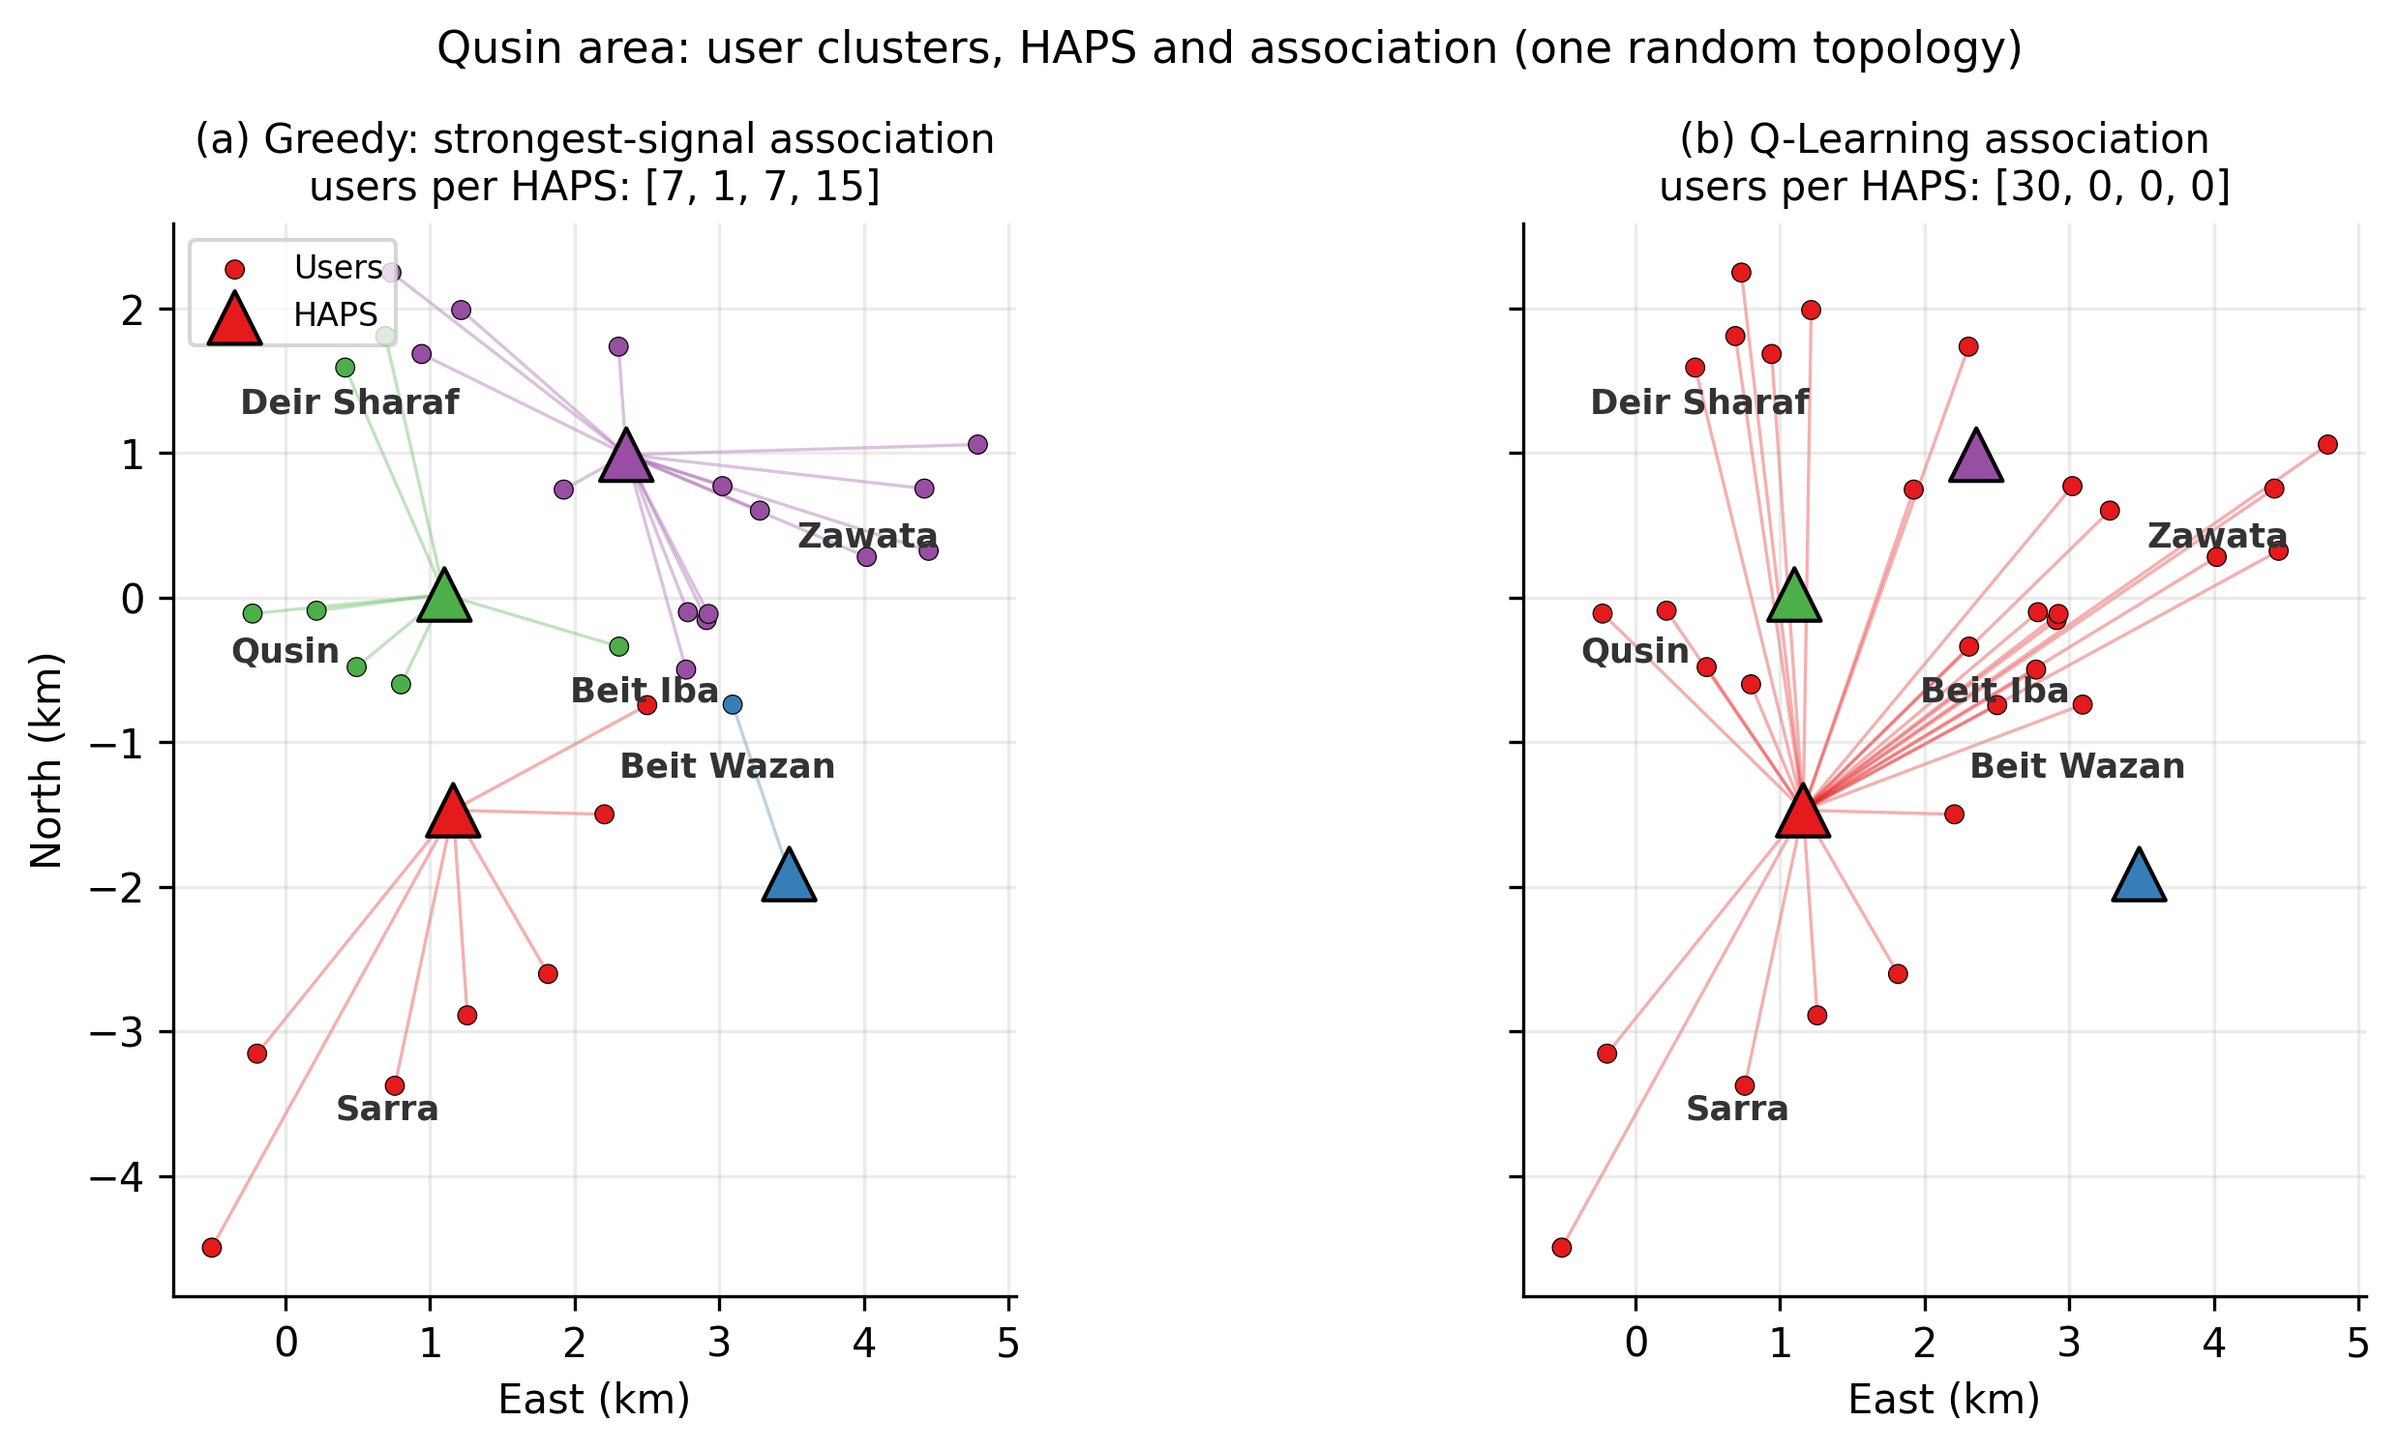
\includegraphics[width=0.78\linewidth]{figures/fig_v1_collapse.png}
\caption{First model, one topology. (a) Greedy association uses all four HAPS. (b) Q-learning puts all 30 users on a single HAPS and leaves the other three idle.}
\label{fig:v1}
\end{figure}

\subsection{Diagnosing the cause}
We tested the natural hypothesis that the satellite backhaul was the bottleneck. It was not: it limited only 2--6\% of users. The real cause is in the radio model. All HAPS reuse the same band with the same antenna gain regardless of direction, and the HAPS are at 20\,km altitude while the whole area is only about 5\,km wide. Seen from any user, the serving HAPS and the other HAPS are therefore at almost the same distance and the same gain, so $\mathrm{SINR}\approx 1/(K-1)$ for $K$ active HAPS: interference swamps the signal. Adding transmitters hurts; switching them off helps. Real HAPS use narrow spot beams, separate frequency sub-bands, and have limited capacity, and none of these is in the toolkit's model. 

\keybox{\textbf{Lesson 1.} A control experiment (\texttt{SingleHAPS}) exposed that the headline result depended on an unrealistic radio model. Always ask: \emph{what trivial strategy could achieve the same thing?}}

%% =====================================================================
\section{Step 4c: Improving the Model}
\label{sec:improve}

We built \texttt{sagin\_v2.py}, which reuses the toolkit's agents, fading, and path loss but replaces the access and backhaul rate computations. There are four changes.

\subsection{Spot beams (access tier)}
A HAPS points a beam at the user it is serving. The desired link gets the peak gain $G$ (35\,dBi by default); interference reaches another user through the beam's pattern, which falls with the angle $\theta$ between the beam direction and the victim user as seen from the HAPS:
\begin{equation}
  A(\theta)=\min\!\Big(12\big(\theta/\theta_{3\mathrm{dB}}\big)^2,\ \mathrm{SLA}\Big)\ \text{dB},\qquad
  \theta_{3\mathrm{dB}}=\sqrt{30000/G_{\mathrm{lin}}}\ \text{degrees},
  \label{eq:pattern}
\end{equation}
with a side-lobe cap $\mathrm{SLA}=25$\,dB. This parabolic main-lobe form is of the same type as the antenna element patterns in 3GPP TR~38.901~\cite{3gpp38901}; we use it as a simple, transparent approximation. With $G=35$\,dBi, $\theta_{3\mathrm{dB}}\approx3.1^\circ$, which is about a 1\,km footprint from 20\,km altitude, so beams can separate neighbouring villages (Figure~\ref{fig:beam}). Beams are scheduled round-robin, so the interference a user sees from HAPS $m$ is the \emph{average} over $m$'s served users.

\begin{figure}[h]
\centering
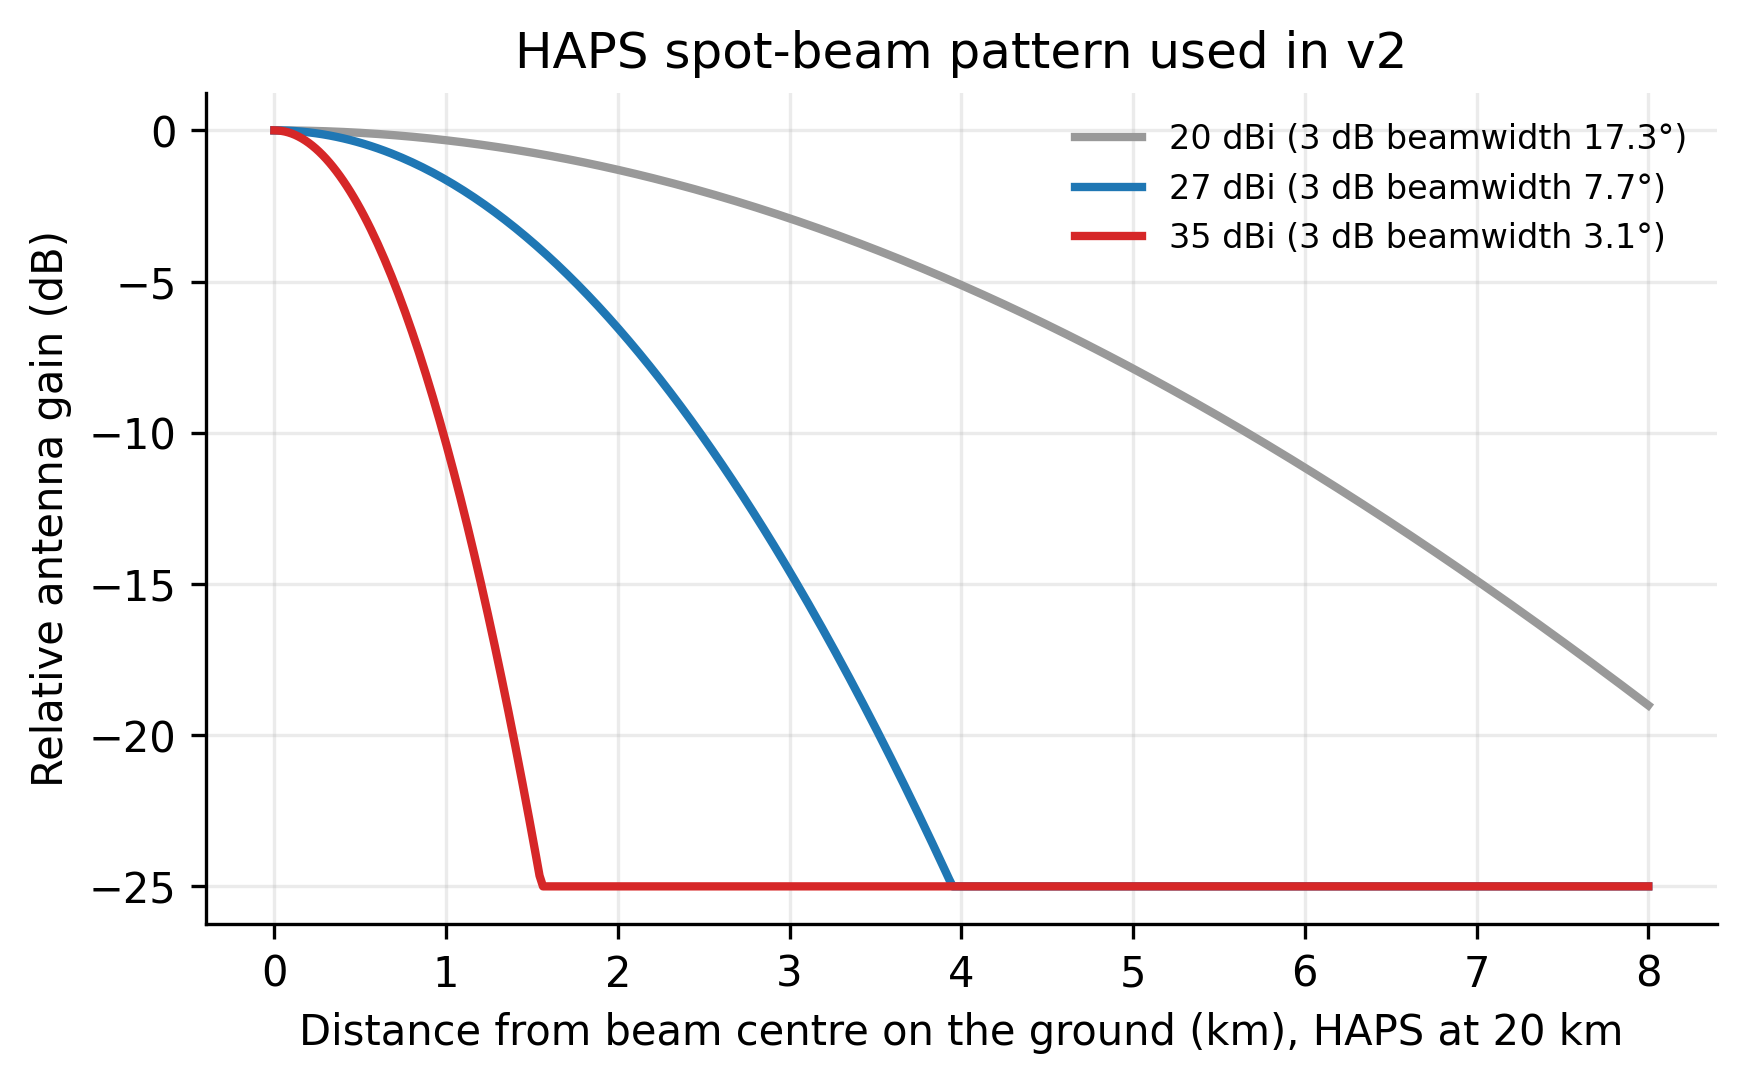
\includegraphics[width=0.62\linewidth]{figures/fig_beam.png}
\caption{Beam pattern used in the improved model for three peak gains. A 20\,dBi beam is almost omnidirectional over the whole area; a 35\,dBi beam separates users about 1--2\,km apart.}
\label{fig:beam}
\end{figure}

\subsection{Frequency reuse}
The band is split into $F$ sub-bands (default $F=2$). Neighbouring HAPS use different sub-bands (alternating along the east--west order), so interference only comes from HAPS in the same sub-band, but each HAPS owns only $B/F$ of the spectrum.

\subsection{Capacity}
A HAPS serves at most $k_{\max}=12$ users; if more are associated, only the 12 strongest are admitted and the rest are \emph{blocked} (rate 0). Q-learning feels the penalty through its reward.

\subsection{Directional backhaul}
This fourth change was discovered during evaluation (Section~\ref{sec:baselines}). The toolkit lets satellites interfere with each other at full strength, so using two LEOs is penalised. In practice each HAPS points a high-gain dish (40\,dBi) at its serving LEO, so we apply the same pattern~\eqref{eq:pattern} to the angular separation of the LEOs as seen from each HAPS.

\subsection{Resulting rate model}
For user $j$ served by HAPS $m=a_j$ and admitted at that HAPS, with $\mathcal{A}_m$ the set of users admitted at $m$,
\begin{align}
  R_j &= \frac{1}{F\,|\mathcal{A}_m|}\log_2\!\big(1+\mathrm{SINR}_j\big),\\
  \mathrm{SINR}_j &= \frac{P_m\, g_{m,j}}{\sum_{m'\neq m,\ f(m')=f(m)} P_{m'}\, g_{m',j}\,\bar\rho_{m',j}+N_0/F},\qquad
  \bar\rho_{m',j}=\frac{1}{|\mathcal{A}_{m'}|}\sum_{i\in\mathcal{A}_{m'}}10^{-A(\theta^{m'}_{ij})/10},
\end{align}
where $f(\cdot)$ is the sub-band. The end-to-end rate is $r_j=\min\{R_j,\ R^{\mathrm{bh}}_{m}/|\mathcal{A}_m|\}$, with $R^{\mathrm{bh}}_m$ the backhaul rate of HAPS $m$ computed in the same way with directional dishes. Blocked users have $r_j=0$. The core of the access computation is only a few lines of NumPy:
\begin{lstlisting}
def access_rates(p_w, assoc, topo, gain, noise_w, p):
    n_h, n_u = gain.shape
    adm = np.zeros((n_h, n_u), dtype=bool)
    for m in range(n_h):                     # admission control
        idx = np.flatnonzero(assoc == m)
        if idx.size > p.kmax:                # keep the strongest
            idx = idx[np.argsort(-topo.pg_haps_gu_db[m, idx])[:p.kmax]]
        adm[m, idx] = True
    n_adm = adm.sum(1)
    mean_rel = np.einsum("mi,mij->mj", adm.astype(float), topo.rel) \
               / np.maximum(n_adm, 1)[:, None]
    imat = p_w[:, None] * gain * mean_rel * (n_adm > 0)[:, None]
    cc = topo.subband[:, None] == topo.subband[None, :]
    j = np.arange(n_u)
    inter = (imat * cc[:, assoc]).sum(0) - imat[assoc, j]
    desired = p_w[assoc] * gain[assoc, j]
    sinr = desired / (inter + noise_w / p.n_sub)
    rate = np.log2(1 + sinr) / p.n_sub / np.maximum(n_adm[assoc], 1)
    return rate * adm[assoc, j], adm[assoc, j], n_adm
\end{lstlisting}

\begin{table}[h]
\centering\small
\begin{tabular}{lll}
\toprule
\textbf{Parameter} & \textbf{Value} & \textbf{Origin}\\
\midrule
Carrier / bandwidth & 2\,GHz / 10\,MHz & toolkit default\\
LEO / HAPS altitude & 300\,km / 20\,km & toolkit default\\
Noise figure & 7\,dB & toolkit default\\
Power codebook & 10 levels, 10--40\,dBm & toolkit default\\
HAPS beam peak gain & 35\,dBi & our assumption\\
Backhaul dish gain & 40\,dBi & toolkit default\\
Side-lobe cap SLA & 25\,dB & our assumption\\
Sub-bands $F$ & 2 & our assumption\\
Capacity $k_{\max}$ per HAPS & 12 users & our assumption\\
Outage threshold & $1\Mbps$ & our assumption\\
Q-learning & $\alpha=0.1,\ \gamma=0.9$, $\epsilon:1\to0.01$ over 60\% of 20\,000 episodes & toolkit default\\
\bottomrule
\end{tabular}
\caption{Parameters of the improved model. Everything marked ``our assumption'' is varied in the sweeps of Section~\ref{sec:results}.}
\label{tab:params}
\end{table}

%% =====================================================================
\section{Step 5: Fair Baselines}
\label{sec:baselines}

A result is only as meaningful as the baselines it is compared with. We use eight methods (Table~\ref{tab:methods}); the last three were added \emph{because of} problems we found.

\begin{table}[h]
\centering\small
\begin{tabular}{p{3.6cm}p{11cm}}
\toprule
\textbf{Method} & \textbf{Description}\\
\midrule
Q-Learning & The toolkit's independent tabular Q-learners (association and power, both tiers).\\
Random & Random associations and powers.\\
MaxPower+Greedy & Strongest-signal association, maximum power.\\
BestUniform+Greedy & Strongest-signal association, one common power chosen to maximise sum-rate.\\
GreedyLB & Strongest users first; each takes its best HAPS that still has room (respects capacity); best common power.\\
GreedyLB+LEO & GreedyLB plus balanced HAPS$\rightarrow$LEO association (at most $\lceil H/L\rceil$ HAPS per LEO).\\
GreedyLB+LEO (minP) & As GreedyLB+LEO but uses the \emph{smallest} common power that keeps topology outage $\le1\%$.\\
SingleHAPS & Control: all users on the best HAPS (respecting the capacity limit, so most are blocked).\\
\bottomrule
\end{tabular}
\caption{Compared methods.}
\label{tab:methods}
\end{table}

\subsection{Why \texttt{GreedyLB}: capacity-aware association}
Strongest-signal association overloads the best HAPS; with a capacity limit the extras are blocked. \texttt{GreedyLB} is the obvious engineering fix and costs a few lines of code.

\subsection{Why \texttt{GreedyLB+LEO}: the satellite-selection discovery}
With strongest-signal LEO association, the HAPS tended to choose the \emph{same} satellite, so one satellite's band was divided four ways. In a diagnostic run on six topologies, all four HAPS picked the same satellite in five of them (three of four in the sixth), and 21 of 21 outage users under \texttt{GreedyLB} were limited by the backhaul, not by the access link. The repository's own README observes that most of Q-learning's advantage comes from tier-1 load balancing~\cite{repo}; our diagnostic is consistent with that, and it means that a baseline without balanced LEO association is unfairly weak.

\subsection{Why \texttt{minP}: an energy-fair baseline}
Choosing the common power that maximises \emph{sum-rate} always ends at the maximum, which wastes energy; comparing a learned policy's power with that is unfair. \texttt{minP} chooses the smallest power that meets the outage target on the given topology. On average it used 7.3\,W (30 users) and 15.1\,W (45 users) in total, against 28.7\,W and 30.0\,W for Q-learning (Table~\ref{tab:main}).

\subsection{Statistics}
Results vary strongly from topology to topology (random user and HAPS placement), so 10 topologies were not enough to rank methods: the same configuration gave 2.0\% and 3.7\% Q-learning outage in two 10-topology runs with different seeds (and a larger swing, 9.0\% vs.\ 4.0\%, in an earlier version of the model). For the headline comparison we use \textbf{30 topologies per load} and report paired differences (Q-learning minus baseline on the same topology) with 95\% bootstrap confidence intervals (5\,000 resamples). Error bars in figures are standard errors across topologies.

\keybox{\textbf{Lesson 2.} Strong, fair baselines and paired statistics are what turn a plot into evidence. The two baselines that changed our conclusions (\texttt{GreedyLB+LEO} and \texttt{minP}) each took only a few lines of code.}

%% =====================================================================
\section{Step 6: Results}
\label{sec:results}

\subsection{Main comparison}
Table~\ref{tab:main} and Figure~\ref{fig:main} show 30 topologies at each of two loads.

\begin{table}[h]
\centering\footnotesize
\resizebox{\linewidth}{!}{%
\begin{tabular}{lrrrrr|rrrrr}
\toprule
 & \multicolumn{5}{c|}{\textbf{30 users}} & \multicolumn{5}{c}{\textbf{45 users}}\\
\textbf{Method} & Sum & P5 & Out. & Power & Blk. & Sum & P5 & Out. & Power & Blk.\\
 & (Mb/s) & (Mb/s) & (\%) & (W) & (\%) & (Mb/s) & (Mb/s) & (\%) & (W) & (\%)\\
\midrule
Q-Learning          & 121.8 & 2.36 &  2.4 & 28.7 & 0.2 & 113.6 & 0.96 & 10.7 & 30.0 &  1.9\\
Random              &  54.9 & 1.47 &  0.0 & 11.7 & 0.5 &  53.3 & 0.96 & 14.5 & 11.8 &  7.5\\
MaxPower+Greedy     &  81.3 & 1.15 &  4.9 & 48.7 & 4.6 &  85.1 & 0.11 & 17.1 & 50.0 & 16.7\\
BestUniform+Greedy  &  81.4 & 1.15 &  5.1 & 48.7 & 4.6 &  85.1 & 0.11 & 17.0 & 50.0 & 16.7\\
GreedyLB            &  83.5 & 1.71 &  0.4 & 49.7 & 0.0 &  83.9 & 1.48 &  0.4 & 50.3 &  0.0\\
GreedyLB+LEO        & 121.1 & 2.29 &  0.2 & 59.7 & 0.0 & 113.8 & 1.73 &  4.6 & 60.3 &  0.0\\
GreedyLB+LEO (minP) &  66.5 & 1.27 &  2.1 &  7.3 & 0.0 &  79.5 & 1.33 &  4.8 & 15.1 &  0.0\\
SingleHAPS          &  22.3 & 0.00 & 60.0 & 20.0 & 60.0 &  22.7 & 0.00 & 73.3 & 20.3 & 73.3\\
\bottomrule
\end{tabular}}
\caption{Main results, mean over 30 random topologies per load (3 LEO, 4 HAPS, 35\,dBi beams, 2 sub-bands, $k_{\max}=12$). Sum = mean sum of end-to-end user rates; P5 = 5th-percentile user rate; Out.\ = outage (users below $1\Mbps$); Blk.\ = blocked users.}
\label{tab:main}
\end{table}

\begin{figure}[h]
\centering
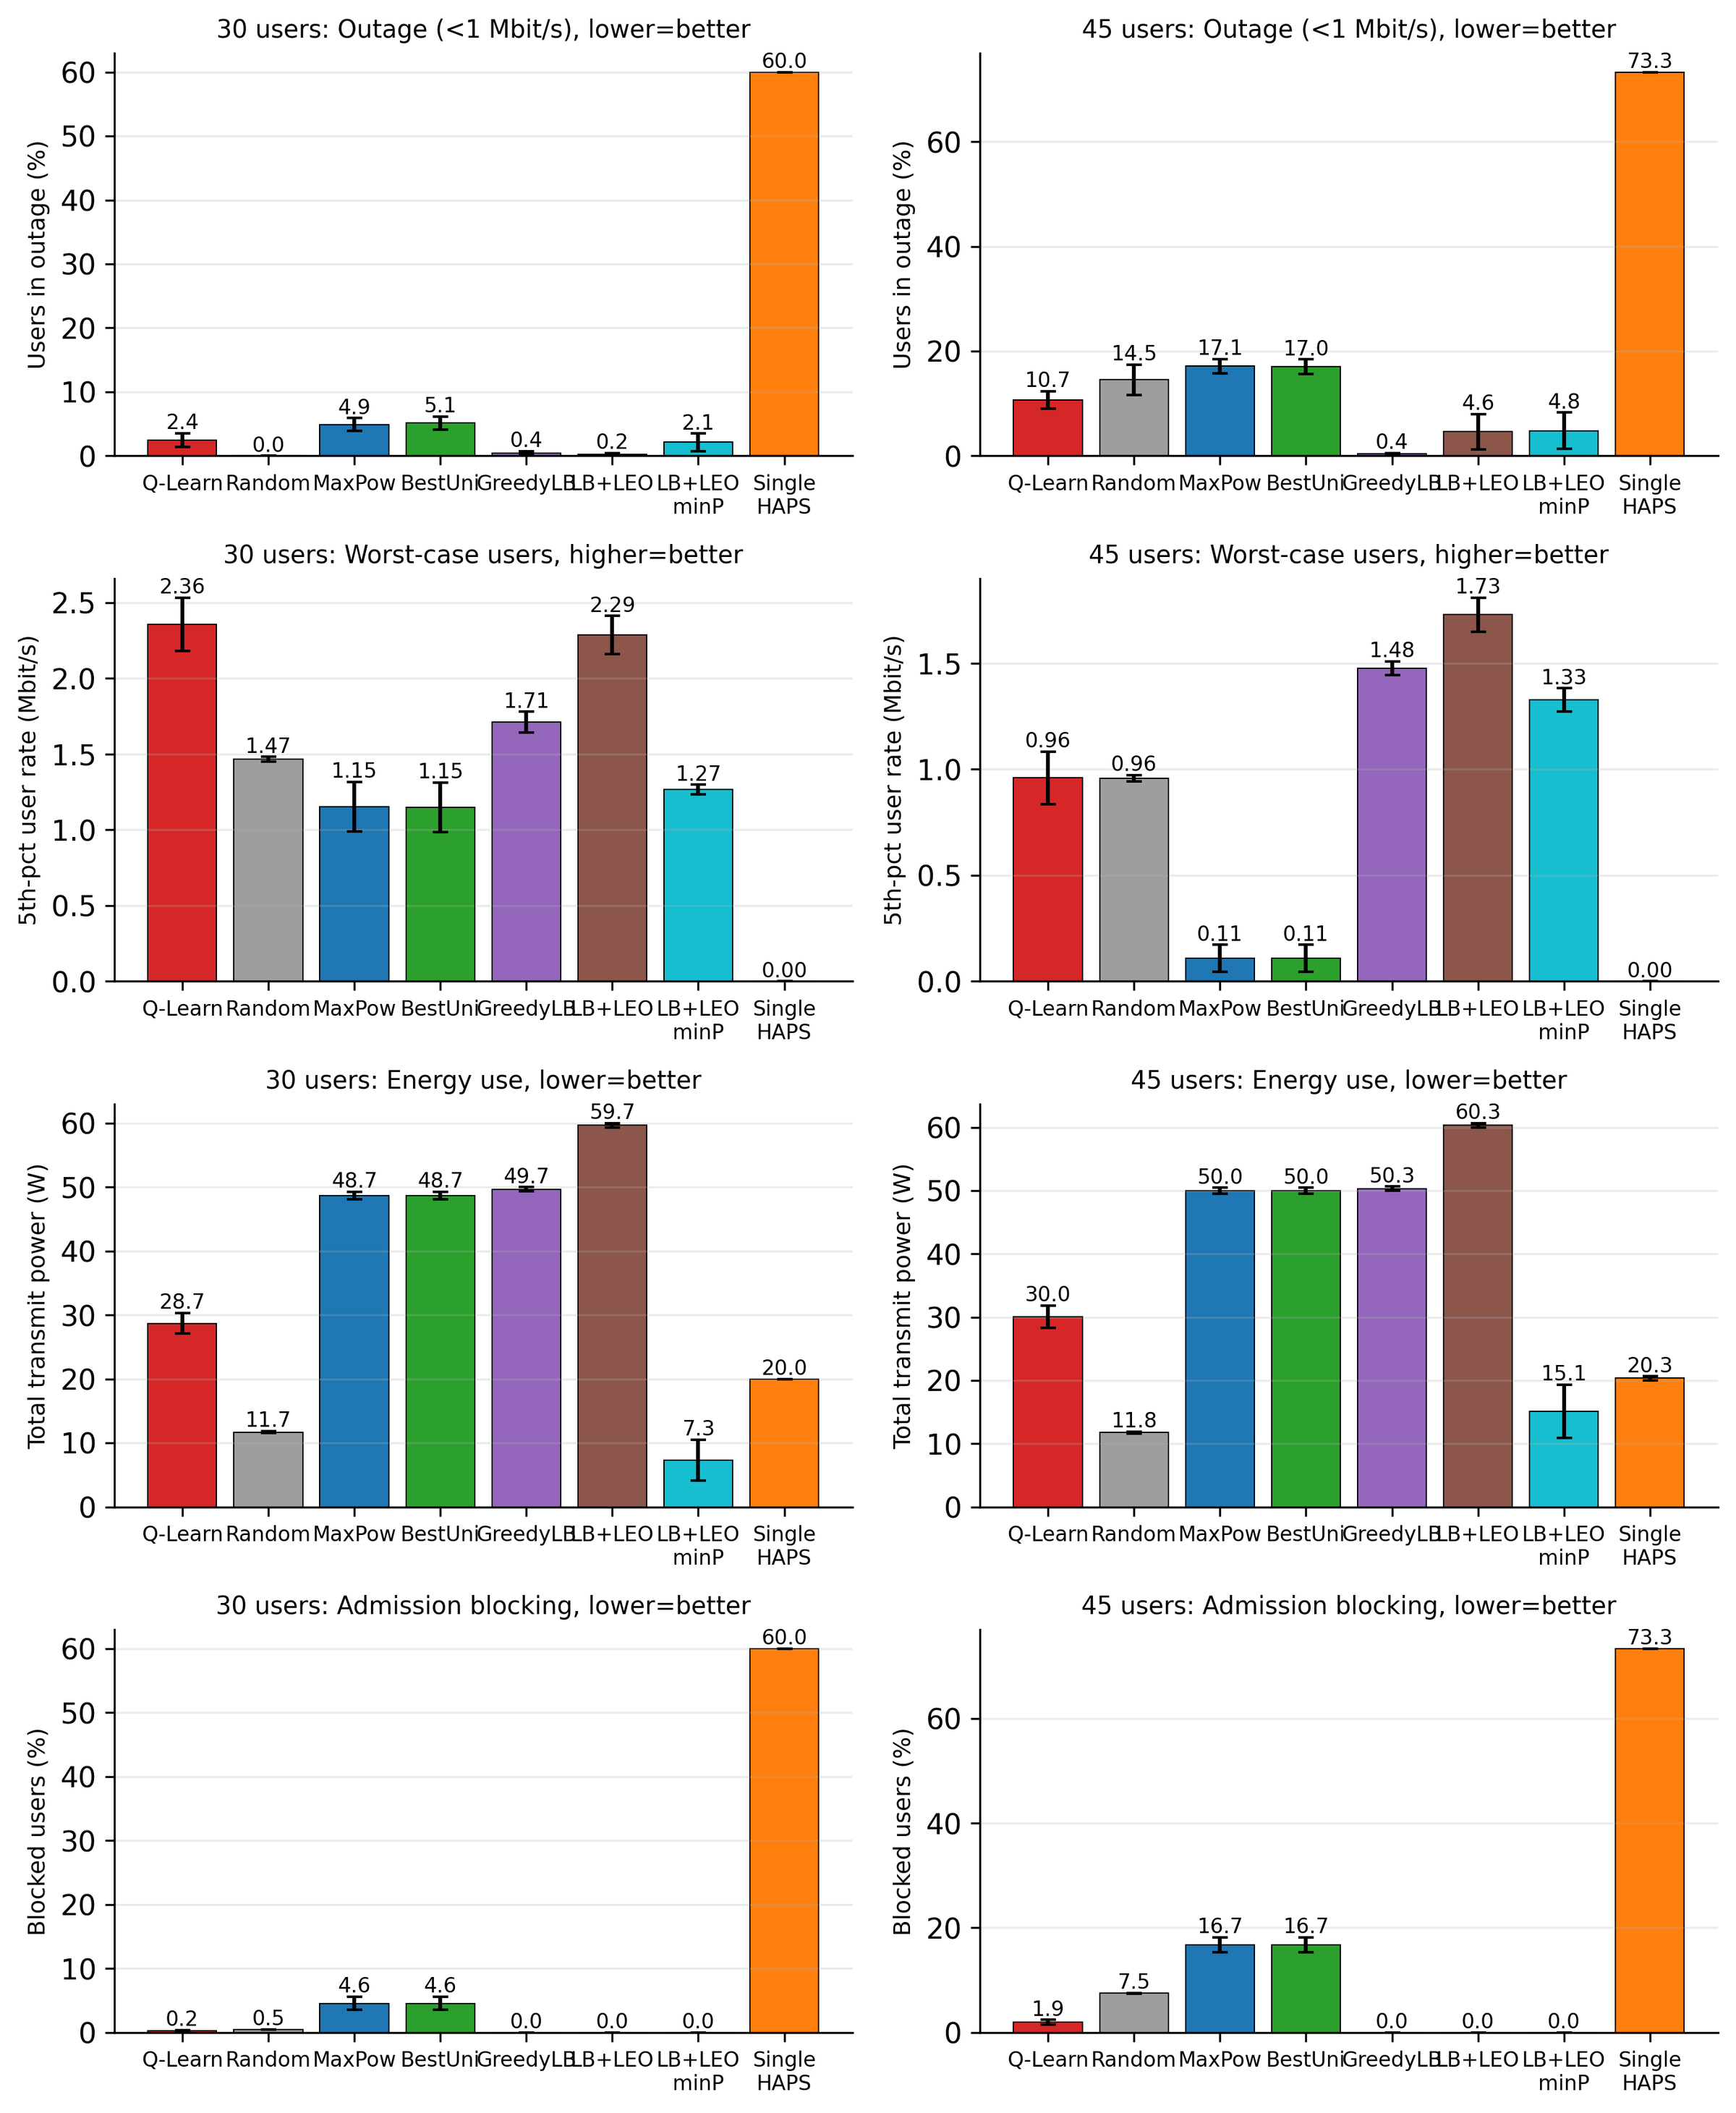
\includegraphics[width=0.9\linewidth]{figures/fig_main.png}
\caption{Main comparison at 30 users (left column) and 45 users (right column); rows show outage, 5th-percentile rate, transmit power and blocking. Error bars are standard errors over 30 topologies.}
\label{fig:main}
\end{figure}

Three observations follow.
\begin{enumerate}
  \item \textbf{At 30 users the load is easy.} Even random association and power meet the $1\Mbps$ threshold for everybody on average. The capacity-blind strategies have about 5\% outage and the one-HAPS control fails badly; differences between the remaining methods are small.
  \item \textbf{At 45 users the methods separate.} Strongest-signal strategies block 17\% of users; \texttt{GreedyLB} has outage 0.4\%; Q-learning 10.7\%.
  \item \textbf{Energy.} Q-learning and the other methods differ strongly in transmit power: about 29--30\,W for Q-learning, 50--60\,W for the rate-maximising baselines, and only 7--15\,W for \texttt{minP}.
\end{enumerate}

\subsection{Paired comparison with confidence intervals}
Table~\ref{tab:paired} reports differences (Q-learning minus baseline) on identical topologies. For outage, power and blocking, negative values favour Q-learning; for rates, positive values do.

\begin{table}[h]
\centering\footnotesize
\resizebox{\linewidth}{!}{%
\begin{tabular}{llrrrr}
\toprule
\textbf{Load} & \textbf{Versus} & \textbf{$\Delta$ outage (pp)} & \textbf{$\Delta$ P5 (Mb/s)} & \textbf{$\Delta$ power (W)} & \textbf{$\Delta$ sum (Mb/s)}\\
\midrule
30 & GreedyLB+LEO (minP) & 0.33 [$-$3.33, 3.22] & 1.09 [0.73, 1.45] & 21.4 [13.8, 27.6] & 55.3 [47.4, 62.4]\\
30 & GreedyLB+LEO & 2.22 [0.22, 4.56] & 0.07 [$-$0.28, 0.43] & $-$31.0 [$-$34.1, $-$27.9] & 0.7 [$-$3.5, 4.6]\\
30 & GreedyLB & 2.00 [0.22, 4.22] & 0.64 [0.30, 0.99] & $-$21.0 [$-$24.2, $-$18.0] & 38.3 [35.1, 41.3]\\
30 & BestUniform+Greedy & $-$2.67 [$-$5.56, 0.44] & 1.21 [0.77, 1.65] & $-$20.0 [$-$23.3, $-$16.7] & 40.4 [37.0, 43.8]\\
\midrule
45 & GreedyLB+LEO (minP) & 5.85 [$-$3.04, 12.59] & $-$0.37 [$-$0.66, $-$0.08] & 14.9 [4.9, 23.8] & 34.2 [24.1, 43.4]\\
45 & GreedyLB+LEO & 6.07 [$-$2.74, 12.67] & $-$0.77 [$-$1.06, $-$0.45] & $-$30.3 [$-$33.8, $-$26.7] & $-$0.2 [$-$7.7, 8.2]\\
45 & GreedyLB & 10.30 [7.11, 13.78] & $-$0.52 [$-$0.78, $-$0.25] & $-$20.3 [$-$24.0, $-$16.6] & 29.7 [23.8, 34.8]\\
45 & BestUniform+Greedy & $-$6.37 [$-$10.52, $-$2.22] & 0.85 [0.62, 1.09] & $-$20.0 [$-$23.6, $-$16.0] & 28.5 [22.5, 33.6]\\
\bottomrule
\end{tabular}}
\caption{Paired differences, Q-learning minus baseline, mean with 95\% bootstrap CI over 30 topologies. pp = percentage points.}
\label{tab:paired}
\end{table}

Reading the table carefully:
\begin{itemize}
  \item \textbf{Versus naive baselines} (\texttt{BestUniform+Greedy}, equivalently \texttt{MaxPower+Greedy}), Q-learning is clearly better at 45 users: outage $-6.4$\,pp (CI excludes zero), 5th-percentile rate $+0.85\Mbps$, power about 20\,W lower.
  \item \textbf{Versus capacity-aware heuristics}, Q-learning is not better on outage. At 45 users it is worse than \texttt{GreedyLB} by 10.3\,pp (CI excludes zero), and worse on the 5th-percentile rate against all three heuristics. At 30 users it is slightly worse on outage than \texttt{GreedyLB} and \texttt{GreedyLB+LEO} (about 2\,pp, CI excludes zero).
  \item \textbf{Versus \texttt{GreedyLB+LEO}}, Q-learning has equal sum-rate (the CI includes zero at both loads) and uses about 30\,W less, but \texttt{GreedyLB+LEO} has lower outage at 30 users (CI excludes zero) and the two are not statistically distinguishable at 45 users.
  \item \textbf{Versus \texttt{minP}}, Q-learning's outage difference is not distinguishable from zero, but \texttt{minP} uses 14.9--21.4\,W less power.
\end{itemize}
We did not investigate why \texttt{GreedyLB+LEO} shows more outage than \texttt{GreedyLB} at 45 users (4.6\% vs.\ 0.4\%) even though its sum-rate is higher; one likely factor is that choosing power to maximise sum-rate does not minimise outage, but we have not tested this explanation.

\subsection{How the learned policy behaves}
Figure~\ref{fig:assoc} shows one topology. The strongest-signal rule overloads one HAPS (15 users for a limit of 12, so 3 are blocked); \texttt{GreedyLB} and Q-learning respect the limit. Q-learning's associations are less intuitive than \texttt{GreedyLB}'s: some users connect to a more distant HAPS, plausibly to keep interference in the shared sub-band low. Figure~\ref{fig:learn} shows convergence: the training reward rises from about 21 to 33.5 and stabilises when exploration ends at episode 12\,000.

\begin{figure}[h]
\centering
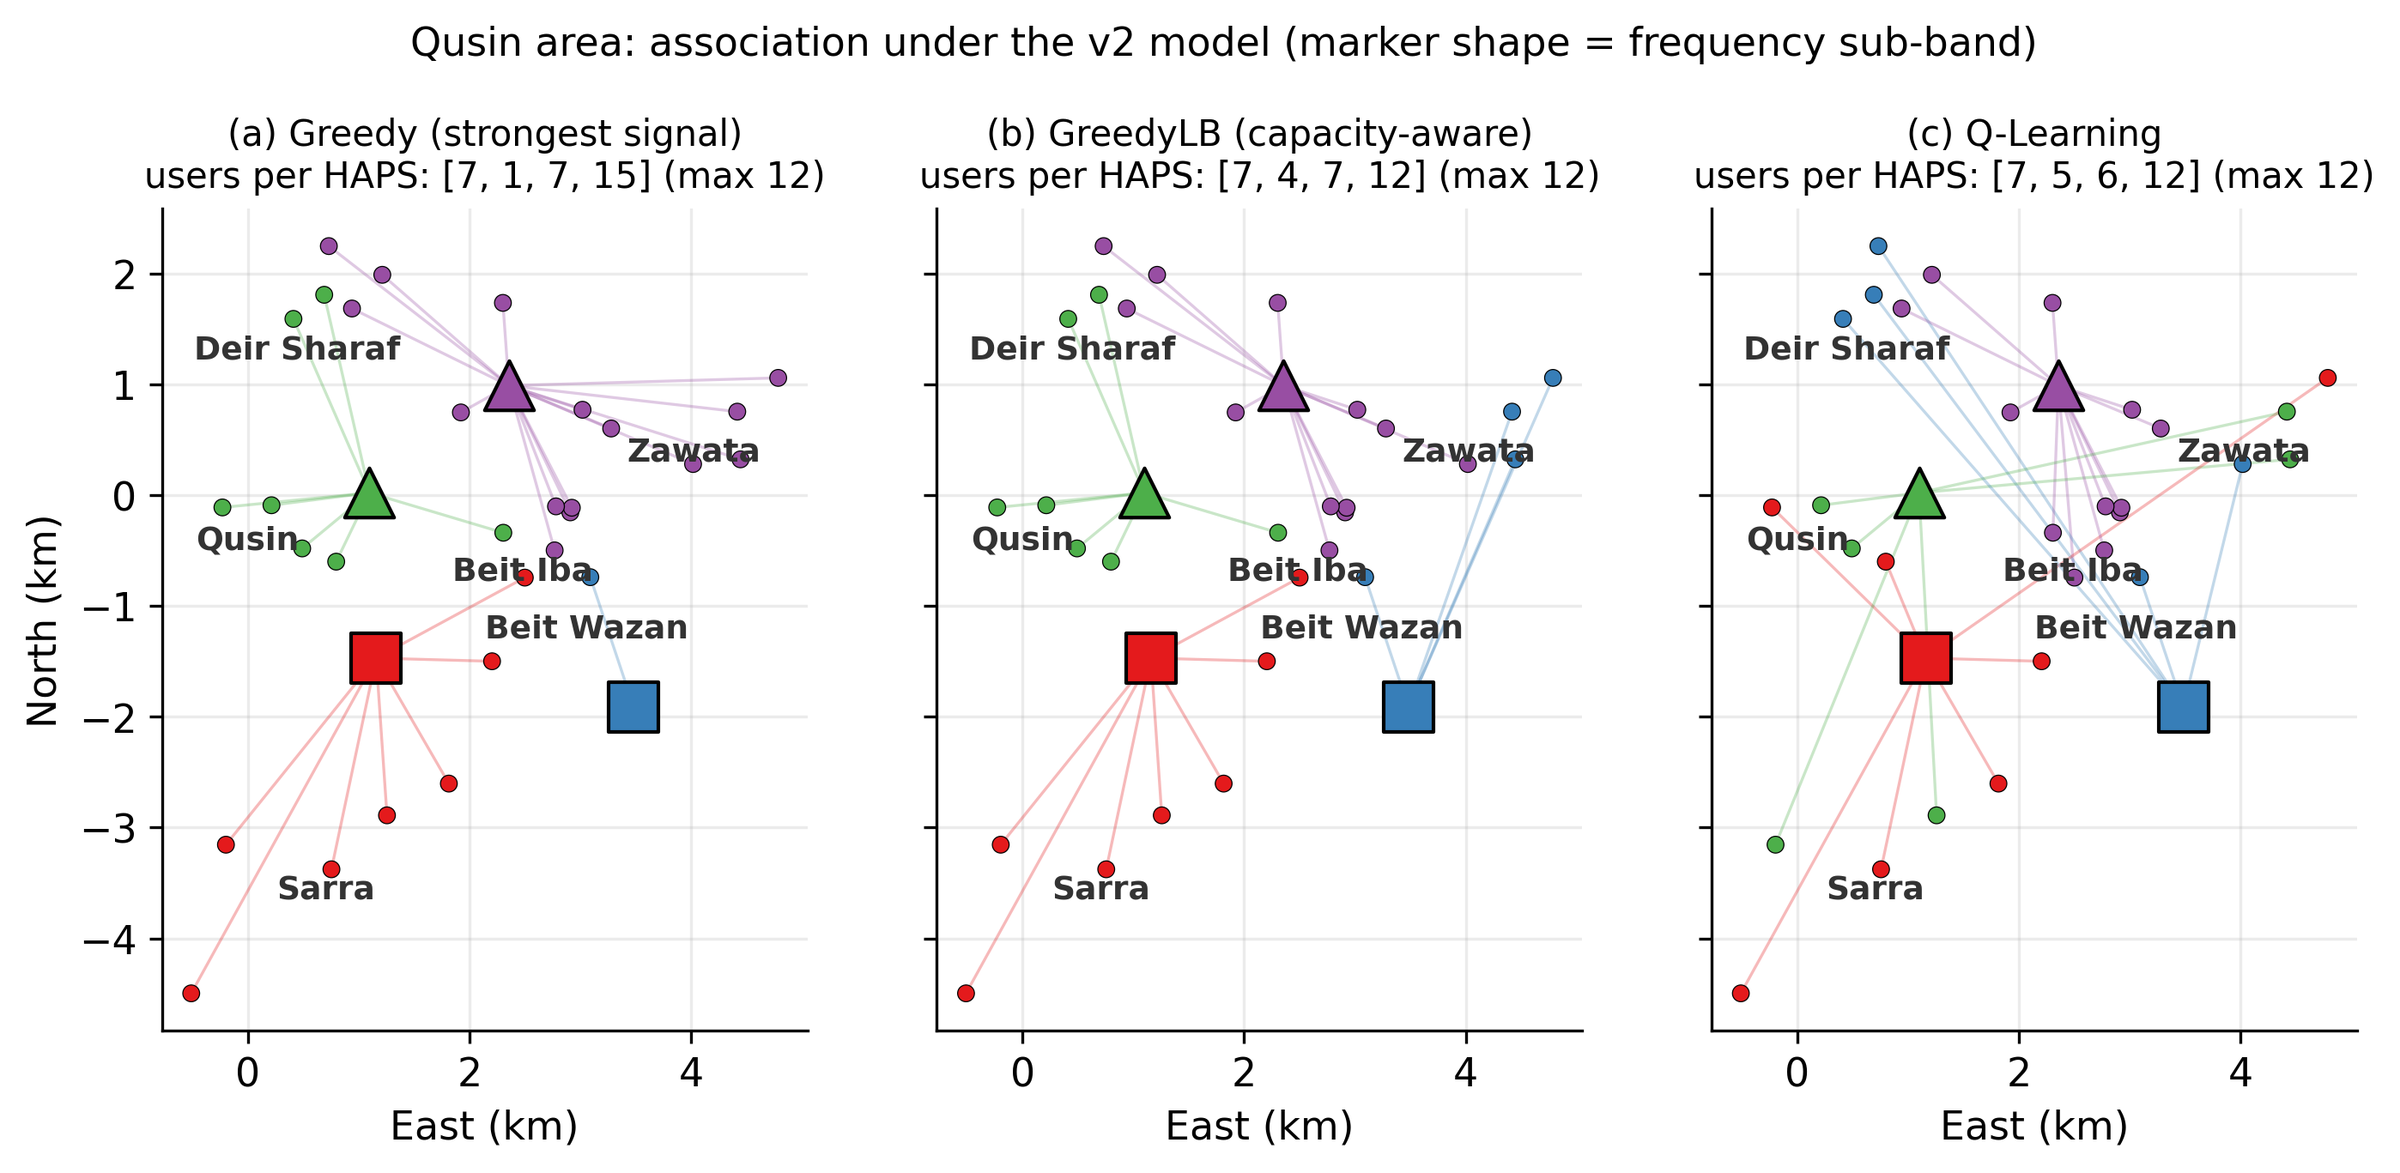
\includegraphics[width=\linewidth]{figures/fig_assoc_v2.png}
\caption{Associations in the improved model for one topology. Colours identify the serving HAPS; marker shape identifies the frequency sub-band.}
\label{fig:assoc}
\end{figure}

\begin{figure}[h]
\centering
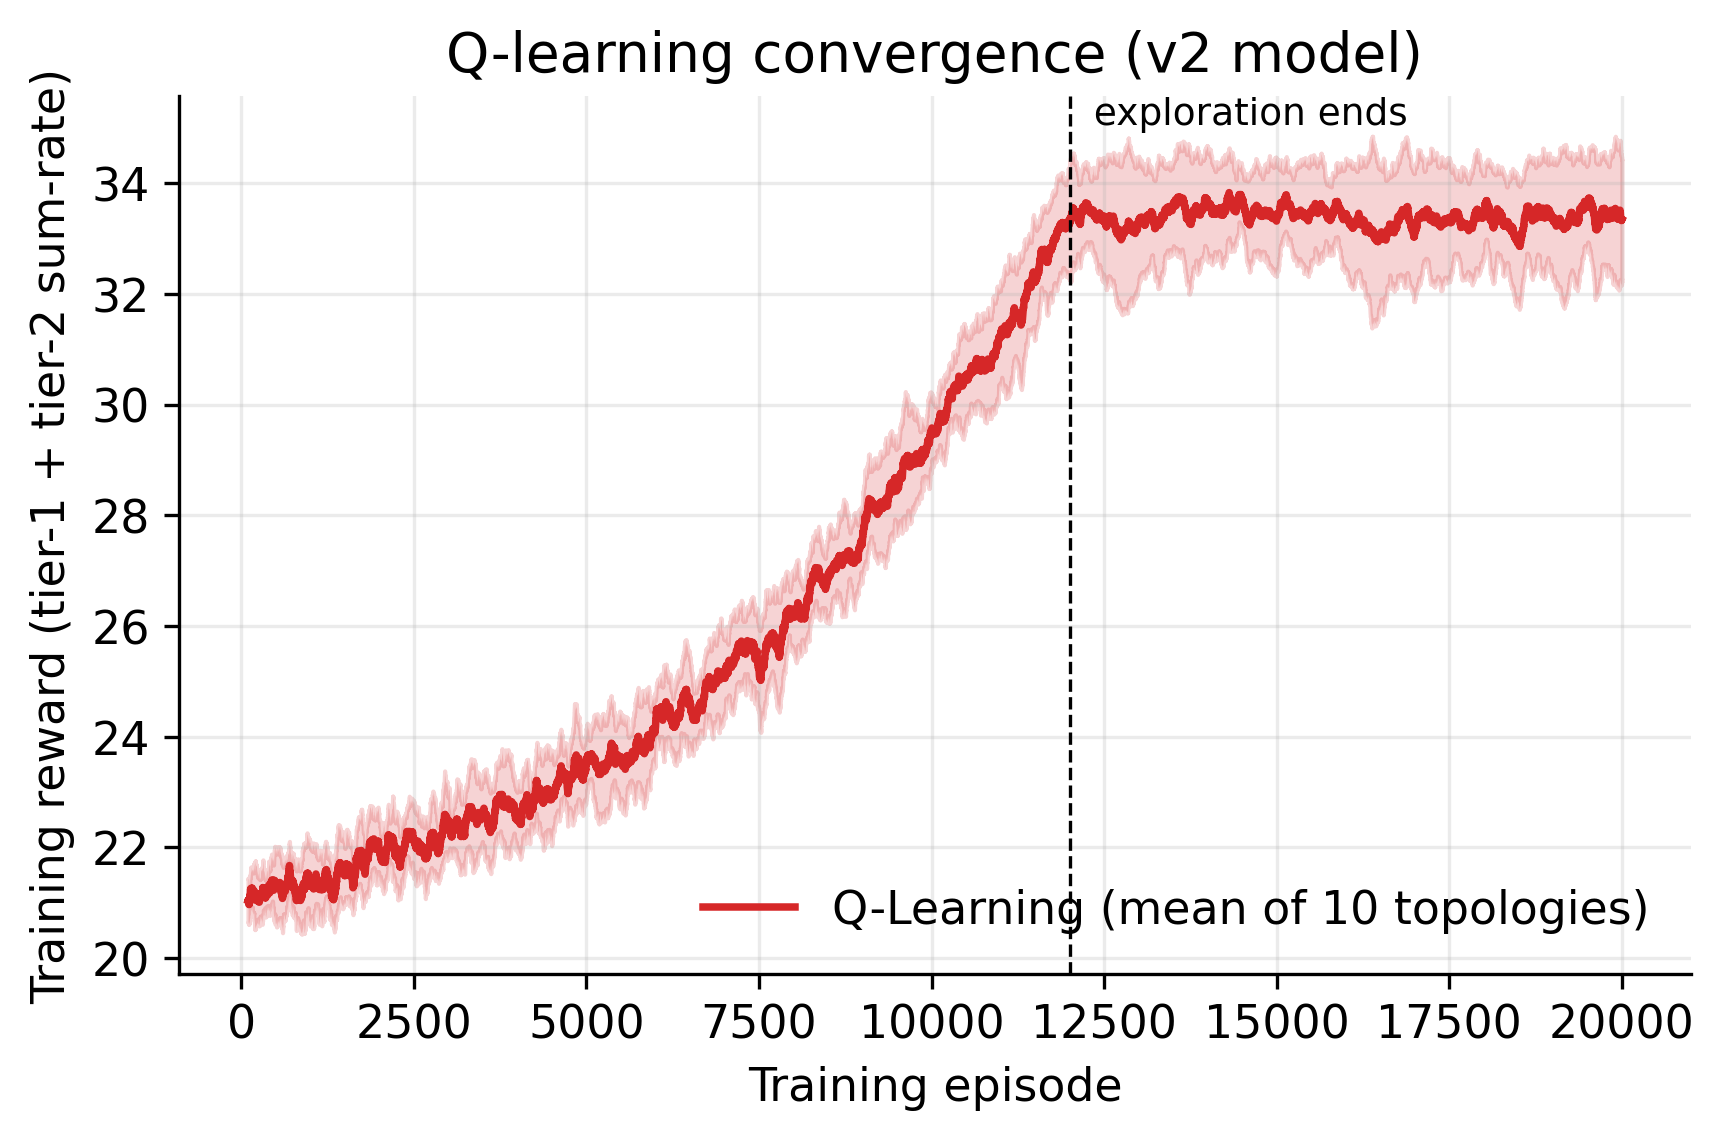
\includegraphics[width=0.6\linewidth]{figures/fig_learning.png}
\caption{Q-learning training reward (mean $\pm$ s.d.\ over 10 topologies, moving average). The dashed line marks the end of exploration.}
\label{fig:learn}
\end{figure}

\subsection{Sensitivity to load, frequency reuse and beam gain}
Figure~\ref{fig:sweeps} and Table~\ref{tab:sweeps} vary one factor at a time (10 topologies per point, so these curves are indicative rather than conclusive).

\begin{figure}[h]
\centering
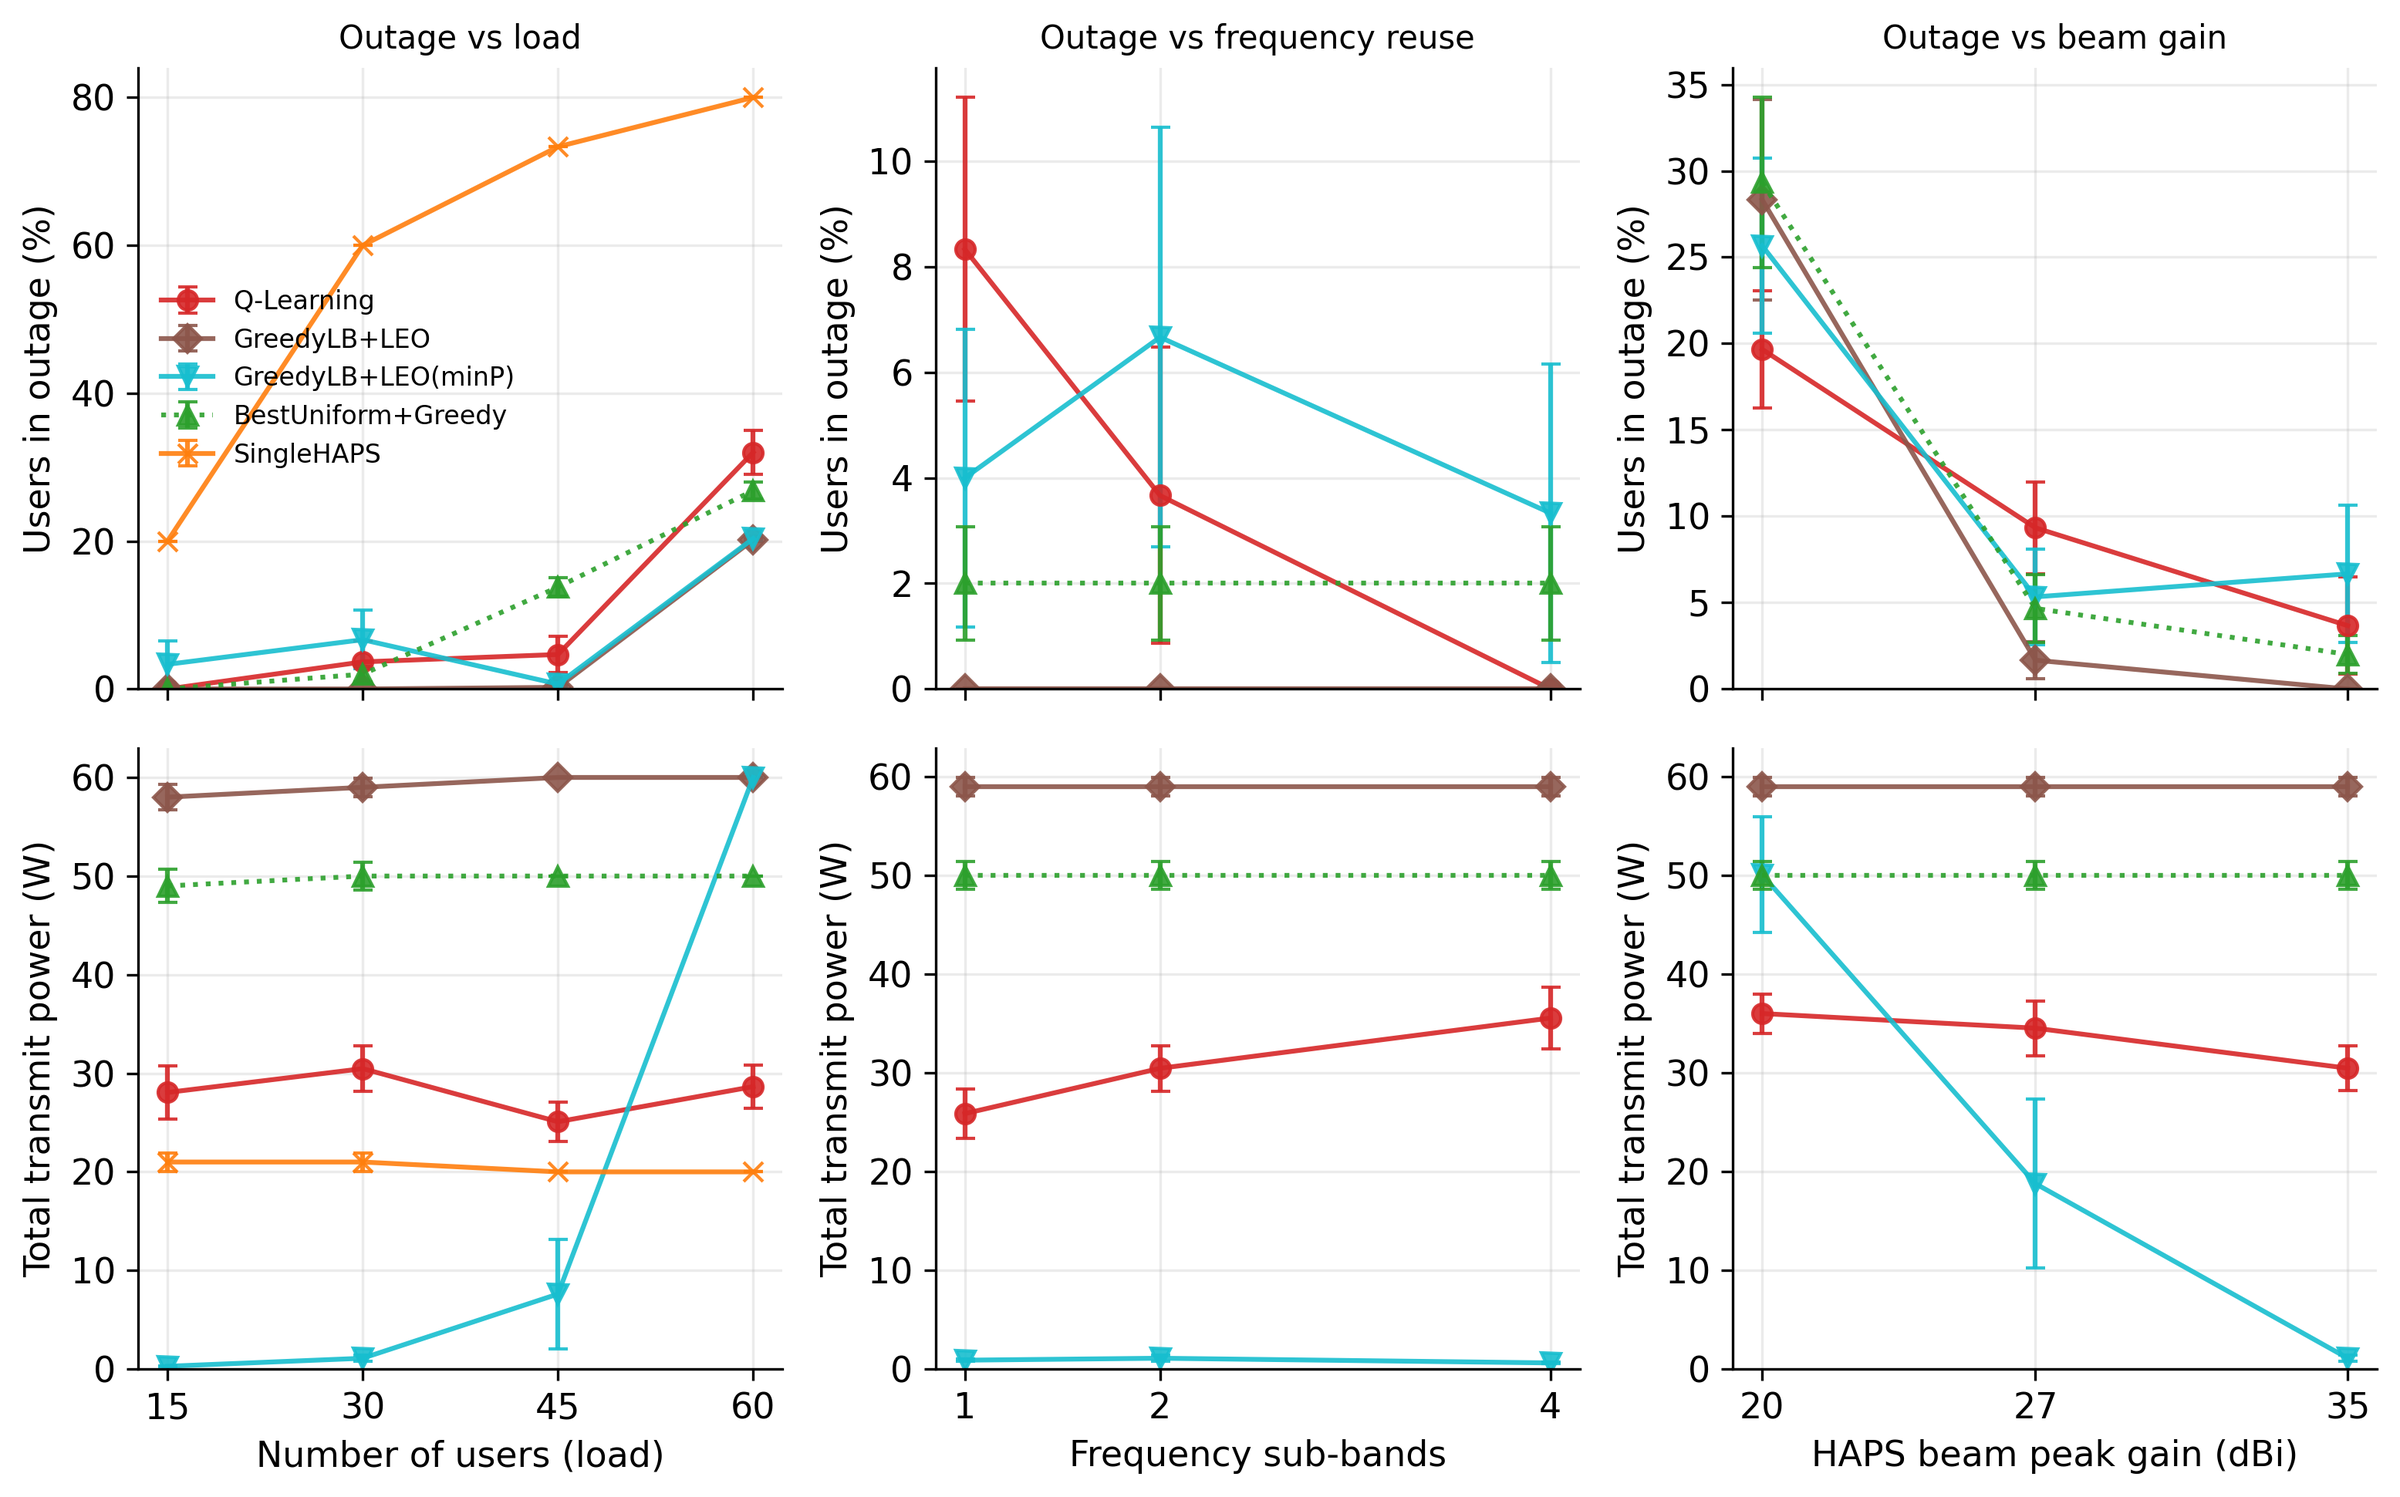
\includegraphics[width=\linewidth]{figures/fig_sweeps.png}
\caption{Outage (top) and transmit power (bottom) versus number of users (left), frequency sub-bands (middle) and HAPS beam gain (right). Error bars are standard errors over 10 topologies.}
\label{fig:sweeps}
\end{figure}

\begin{table}[h]
\centering\footnotesize
\resizebox{\linewidth}{!}{%
\begin{tabular}{lrrrr|rrr|rrr}
\toprule
 & \multicolumn{4}{c|}{\textbf{Users}} & \multicolumn{3}{c|}{\textbf{Sub-bands $F$}} & \multicolumn{3}{c}{\textbf{Beam gain (dBi)}}\\
\textbf{Outage (\%)} & 15 & 30 & 45 & 60 & 1 & 2 & 4 & 20 & 27 & 35\\
\midrule
Q-Learning          & 0.0 & 3.7 & 4.7 & 32.0 & 8.3 & 3.7 & 0.0 & 19.7 & 9.3 & 3.7\\
GreedyLB            & 0.0 & 0.0 & 0.2 & 20.3 & 0.0 & 0.0 & 0.0 & 31.3 & 3.0 & 0.0\\
GreedyLB+LEO        & 0.0 & 0.0 & 0.2 & 20.2 & 0.0 & 0.0 & 0.0 & 28.3 & 1.7 & 0.0\\
GreedyLB+LEO (minP) & 3.3 & 6.7 & 0.7 & 20.3 & 4.0 & 6.7 & 3.3 & 25.7 & 5.3 & 6.7\\
BestUniform+Greedy  & 0.0 & 2.0 & 13.8 & 26.8 & 2.0 & 2.0 & 2.0 & 29.3 & 4.7 & 2.0\\
SingleHAPS          & 20.0 & 60.0 & 73.3 & 80.0 & -- & -- & -- & -- & -- & --\\
\bottomrule
\end{tabular}}
\caption{Outage (\%) in the sensitivity sweeps (10 topologies per point; the baseline point is 30 users, $F=2$, 35\,dBi).}
\label{tab:sweeps}
\end{table}

\begin{itemize}
  \item \textbf{Load.} Up to 30 users every sensible method serves nearly everybody. At 60 users demand exceeds the capacity of four HAPS with $k_{\max}=12$ (48 slots), so even the best methods have about 20\% outage, and Q-learning is worse (32\%).
  \item \textbf{Frequency reuse.} More sub-bands help Q-learning (8.3\% $\rightarrow$ 0.0\%), while they barely change the heuristics, whose outage is already at or near zero. Q-learning also uses more power with more sub-bands (25.9 $\rightarrow$ 35.6\,W).
  \item \textbf{Beam gain.} This is the dominant factor. At 20\,dBi, every method has 20--31\% outage; Q-learning is the best in that regime (19.7\% vs.\ 25.7--31.3\%). At 27 and 35\,dBi \texttt{GreedyLB} and \texttt{GreedyLB+LEO} overtake it.
\end{itemize}

%% =====================================================================
\section{Discussion}
\label{sec:discussion}

\subsection{What we learned about the problem}
\begin{enumerate}
  \item \textbf{Hardware first, algorithm second.} Antenna directivity changes outage from roughly 30\% to near 0, more than any choice of algorithm.
  \item \textbf{Respect capacity.} Letting a HAPS take more users than it can serve is the largest avoidable loss: capacity-blind baselines block 17\% of users at 45 users.
  \item \textbf{Balance the backhaul.} Assigning HAPS to different satellites doubles the backhaul share compared with all HAPS using one satellite.
  \item \textbf{Power can be small.} When beams are good, a uniform power as low as 7--15\,W in total (with the minP heuristic) can keep average outage in single digits at these loads.
\end{enumerate}

\subsection{What we learned about the tool}
Q-learning is a reasonable, easy-to-run baseline that clearly beats naive strategies, and it can be better than heuristics when the radio environment is poor (20\,dBi). Under good conditions, simple capacity-aware heuristics are as good or better on outage and use less power. Because the toolkit's reward is the sum-rate, it does not directly target outage; the learned policy therefore can have a worse worst-case than a heuristic. A natural next experiment is to reward outage reduction directly (for example, a reward based on the minimum rate or the fraction of users above $1\Mbps$). We did not run this, so we make no claim about its outcome.

\subsection{Limitations and threats to validity}
\begin{itemize}
  \item \textbf{Assumptions.} Beam gain, side-lobe cap, sub-band count, per-HAPS capacity, the $1\Mbps$ threshold and the user spread are assumptions. Results at the other values are in Figure~\ref{fig:sweeps}, but the sweeps use only 10 topologies.
  \item \textbf{Representative users.} 30 and 45 are abstractions of a population of about 16\,500; real traffic is bursty and heterogeneous.
  \item \textbf{Simplified physics.} No mobility, rain or terrain, no scheduling beyond equal sharing and round-robin beam hopping, no regulatory limits, LEO altitude of 300\,km (low compared with many real constellations), and a constant HAPS position with jitter.
  \item \textbf{One learner family.} Only tabular independent Q-learning was tested; other learners may behave differently.
  \item \textbf{Unexplained effects.} We did not investigate why \texttt{GreedyLB+LEO} has more outage than \texttt{GreedyLB} at 45 users.
  \item \textbf{No claim about real infrastructure.} The study says nothing about the actual condition of any network in Qusin or the neighbouring villages; it is a thought experiment on a realistic layout.
\end{itemize}

\subsection{Pitfalls we hit (and how to avoid them)}
\begin{enumerate}
  \item \emph{Trusting a result without a control.} \texttt{SingleHAPS} exposed the model flaw; run the simplest possible alternative before believing a gain.
  \item \emph{Weak baselines.} Greedy satellite selection made all baselines look worse than they should; diagnose \emph{why} a baseline loses.
  \item \emph{Too few random topologies.} Use many topologies and paired statistics; our 10-topology numbers moved noticeably between seeds.
  \item \emph{Units.} Kilometres versus metres caused the original code's path-loss errors; convert units in one place.
  \item \emph{Saving objects.} Python objects (for example a dataclass) pickled from a script run as \texttt{\_\_main\_\_} cannot be unpickled elsewhere unless the class is imported under the same name; keep configuration classes in importable modules.
\end{enumerate}

%% =====================================================================
\section{Reproducibility}
\label{sec:repro}

All code is in four files placed next to the repository files (the repository itself is unmodified): \texttt{qusin\_scenario.py} (villages and clustered layout), \texttt{sagin\_v2.py} (improved model, Q-learning training, baselines, experiment runner), \texttt{paired\_stats.py} (30-topology paired comparison) and \texttt{make\_figures\_v2.py} (figures).
\begin{lstlisting}
# 1. get the toolkit and the four extra files in the same folder
git clone https://github.com/Lewis-panda/Optimizing-SAGIN-Association-Link-Power-Using-Reinforcement-Learning.git sagin
cd sagin && pip install -r requirements.txt
python tests.py                       # toolkit tests

# 2. run
python sagin_v2.py                    # main run + three sweeps, 10-15 min
python paired_stats.py                # 30-topology paired stats, ~10 min
python make_figures_v2.py             # figures
python sagin_v2.py --quick            # short smoke test
\end{lstlisting}
Random seeds are fixed in the scripts (\texttt{--seed} for the main run; $777+n$ for the paired runs), so reruns give identical numbers on the same library versions. Outputs are written to \texttt{results\_qusin\_v2/} (\texttt{summary.txt}, \texttt{paired\_stats.txt}, \texttt{run\_log.txt}, figures). Run times above are for a standard cloud CPU instance; no GPU is needed.

%% =====================================================================
\section{Conclusion}
\label{sec:conclusion}

We followed a complete workflow: pick a repository from a GitHub topic, understand it, tie it to a local problem---an emergency fall-back network for Qusin and its neighbouring villages---run it, and evaluate honestly. The most valuable outcome is a method, not a number. A control experiment showed that the toolkit's default radio model made ``switch everything off but one HAPS'' optimal; a more realistic model with spot beams, frequency reuse, capacity and directional backhaul changed the picture; and fair baselines and paired statistics showed that reinforcement learning is better than naive strategies but not better than simple, well-designed heuristics on outage, and that antenna directivity matters more than either. We hope this tutorial lets a reader repeat the work in a day and, more importantly, ask the same sceptical questions about any tool they pick up next.

\section*{Acknowledgements and AI-assistance statement}
Code and text drafting in this project were carried out with the assistance of an AI model (Claude, by Anthropic); the author reviewed the work and is responsible for its content. The toolkit used is the work of its GitHub maintainer, \texttt{Lewis-panda}.

%% =====================================================================
\begin{thebibliography}{99}\small

\bibitem{repo} Lewis-panda, ``Optimizing-SAGIN-Association-Link-Power-Using-Reinforcement-Learning,'' GitHub repository, 2023--2026. \url{https://github.com/Lewis-panda/Optimizing-SAGIN-Association-Link-Power-Using-Reinforcement-Learning}. Accessed October 2026.

\bibitem{iqbal2021tutorial} S.~Iqbal and J.~M.~Hamamreh, ``A Comprehensive Tutorial on How to Practically Build and Deploy 5G Networks Using Open-Source Software and General-Purpose, Off-the-Shelf Hardware,'' \emph{RS Open Journal on Innovative Communication Technologies}, vol.~2, no.~6, 2021. doi:10.46470/03d8ffbd.4ccb7950.

\bibitem{alsharoa2022} A.~Alsharoa and M.-S.~Alouini, ``Joint User Association and Beamforming in Integrated Satellite-HAPS-Ground Networks,'' \emph{IEEE Trans.\ Wireless Commun.}; arXiv:2204.13257, 2022. (As cited in the repository README.)

\bibitem{mlsched2022} ``Machine Learning-Based User Scheduling in Integrated Satellite-HAPS-Ground Networks,'' arXiv:2205.13958. (As cited in the repository README.)

\bibitem{dqlhaps2022} ``Deep Q-Learning-Based Transmission Power Control of a HAPS with Spectrum Sharing,'' \emph{Sensors}, vol.~22, no.~4, art.~1630, MDPI, 2022. (As cited in the repository README.)

\bibitem{interplay2024} ``On the Interplay of AI and SAGIN,'' arXiv:2402.00881. (Survey, as cited in the repository README.)

\bibitem{sutton2018} R.~S.~Sutton and A.~G.~Barto, \emph{Reinforcement Learning: An Introduction}, 2nd ed., MIT Press, 2018.

\bibitem{3gpp38901} 3GPP, ``Study on channel model for frequencies from 0.5 to 100 GHz,'' TR~38.901. (Parabolic main-lobe antenna pattern of the same form as Eq.~\eqref{eq:pattern}.)

\bibitem{pcbs} Palestinian Central Bureau of Statistics, 2017 Population, Housing and Establishment Census (preliminary results), as reported on the public Wikipedia pages for Qusin, Deir Sharaf, Beit Iba, Sarra (Nablus), Zawata and Beit Wazan. Accessed October 2026.

\end{thebibliography}

\end{document}
